\documentclass[tikz,border=8pt]{standalone}
% Shared look for every TikZ diagram. Load with \input{../../tools/tikz-style.tex}
\usepackage[T1]{fontenc}
\usepackage{lmodern}
\renewcommand{\sfdefault}{lmr}  % diagrams use the same serif as the text
\usetikzlibrary{arrows.meta, positioning, shapes.geometric, calc, fit, backgrounds}
\definecolor{cblue}{HTML}{4C78A8}
\definecolor{corange}{HTML}{F58518}
\definecolor{cgreen}{HTML}{54A24B}
\definecolor{cred}{HTML}{E45756}
\definecolor{cpurple}{HTML}{B279A2}
\definecolor{cgrey}{HTML}{6B6B6B}
\tikzset{
  every picture/.style={font=\sffamily, line width=1.2pt},
  box/.style={draw=#1, fill=#1!12, rounded corners=4pt, align=center, inner sep=7pt, minimum height=1.1cm},
  box/.default=cgrey,
  arrow/.style={-{Stealth[length=3mm]}, draw=cgrey, line width=1.4pt},
  title/.style={font=\sffamily\bfseries\Large},
  note/.style={font=\sffamily\small, text=cgrey, align=center},
}
\AtBeginDocument{\hyphenpenalty=10000 \exhyphenpenalty=10000}

\begin{document}
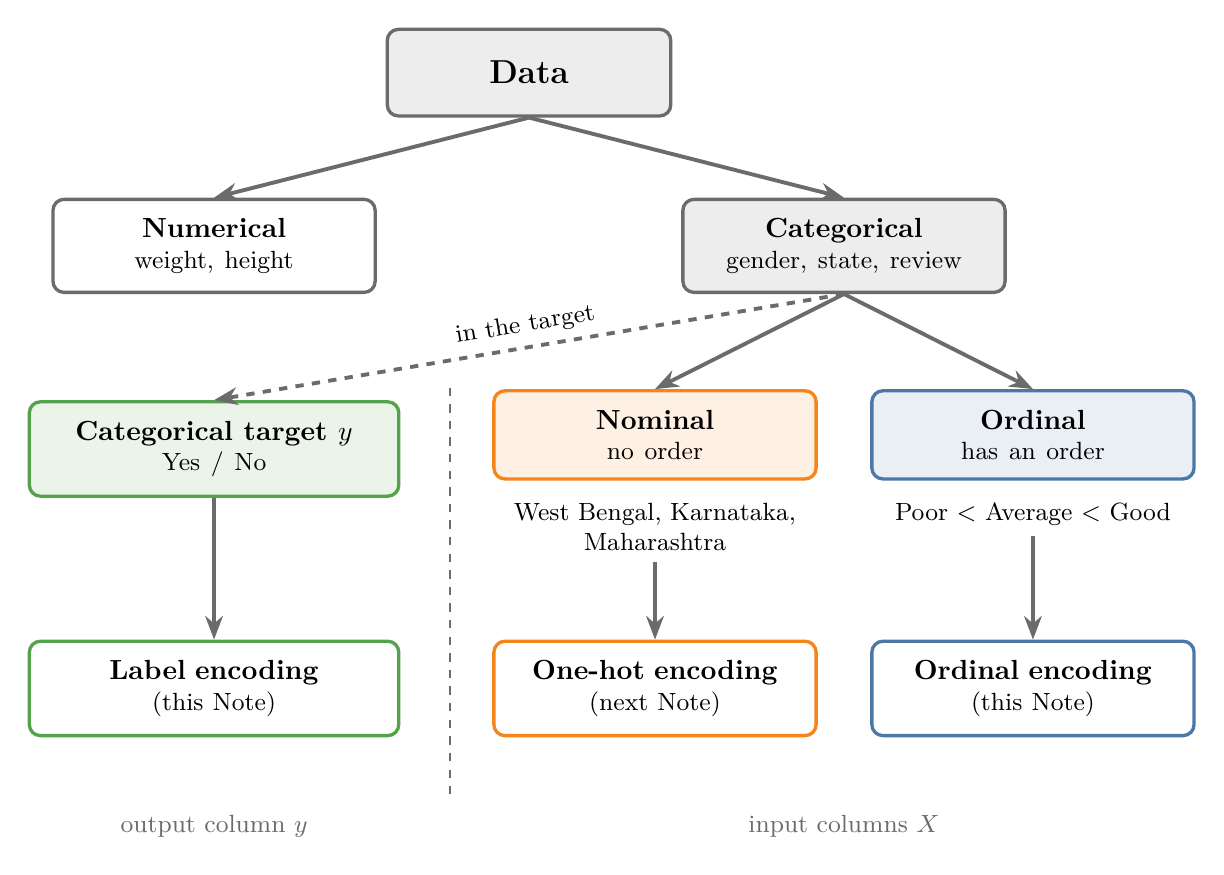
\begin{tikzpicture}
  \node[box=cgrey, font=\sffamily\bfseries\large, minimum width=3.6cm] (d) at (4,0) {Data};
  \node[box=cgrey, fill=white, font=\sffamily\bfseries, text width=3.6cm] (num) at (0,-2.2) {Numerical\\[-1pt]\normalfont\small weight, height};
  \node[box=cgrey, font=\sffamily\bfseries, text width=3.6cm] (cat) at (8,-2.2) {Categorical\\[-1pt]\normalfont\small gender, state, review};
  \draw[arrow] (d.south) -- (num.north);
  \draw[arrow] (d.south) -- (cat.north);
  \node[box=corange, font=\sffamily\bfseries, text width=3.6cm] (nom) at (5.6,-4.6) {Nominal\\[-1pt]\normalfont\small no order};
  \node[box=cblue, font=\sffamily\bfseries, text width=3.6cm] (ord) at (10.4,-4.6) {Ordinal\\[-1pt]\normalfont\small has an order};
  \draw[arrow] (cat.south) -- (nom.north);
  \draw[arrow] (cat.south) -- (ord.north);
  \node[note, text=black, below=0.15cm of nom, text width=3.8cm] (nomx) {West Bengal, Karnataka,\\ Maharashtra};
  \node[note, text=black, below=0.15cm of ord, text width=3.8cm] (ordx) {Poor $<$ Average $<$ Good};
  \node[box=corange, fill=white, text width=3.6cm, anchor=north] (ohe) at (5.6,-7.2) {\textbf{One-hot encoding}\\[-1pt]\small (next Note)};
  \node[box=cblue, fill=white, text width=3.6cm, anchor=north] (oe) at (10.4,-7.2) {\textbf{Ordinal encoding}\\[-1pt]\small (this Note)};
  \draw[arrow] (nomx.south) -- (ohe.north);
  \draw[arrow] (ordx.south) -- (oe.north);
  % target branch
  \node[box=cgreen, fill=white, text width=4.2cm, anchor=north] (lab) at (0,-7.2) {\textbf{Label encoding}\\[-1pt]\small (this Note)};
  \node[box=cgreen, font=\sffamily\bfseries, text width=4.2cm, anchor=south] (tgt) at (0,-5.4) {Categorical target $y$\\[-1pt]\normalfont\small Yes / No};
  \draw[arrow] (tgt.south) -- (lab.north);
  \draw[arrow, dashed] (cat.south) -- node[note, text=black, above, sloped] {in the target} (tgt.north);
  \draw[cgrey, dashed, line width=0.8pt] (3.0,-4.0) -- (3.0,-9.2);
  \node[note, anchor=north] at (8,-9.3) {input columns $X$};
  \node[note, anchor=north] at (0,-9.3) {output column $y$};
\end{tikzpicture}
\end{document}
